\subsection{Nuclear Waste in the United Kingdom}
\label{Nuclear Waste in the United Kingdom SubSection}

The United Kingdom generates 19\%-20\% of its electricity from eight nuclear reactors, though more are currently under construction to be operational by 2026-2030, half of its current power generation is set to be retired by 2025. Magnox Ltd which mainly supplies these nuclear reactors utilise AGR (Advanced Gas-cooled Reactors) that use graphite as its neutron moderator to slow down the fast neutrons so that the nuclear fission can take place and the coolant used is an inert gas such as carbon dioxide or helium. \\

Nuclear waste comes form all sectors across the U.K, however nuclear facilities produce the most waste and when a nuclear reactor is decommissioned due to aging or another hazard that poses serious risk, the materials on site are classed as HAW (Higher Activity Waste) and HLW/ILW (High/ Low Level Waste) as described in \cref{Types of Nuclear Waste SubSection}. When nuclear waste is classified or put into categories the waste is then held at the facilities until transport routes can be determined where the waste will be transported to a recycling or re-processing facility or a storage facility. Nuclear waste that is classified as ILW or HLW must be store for years if not decades until safe to dispose of, this is due to the amount of radioactivity that the materials and objects encounter. HLW is sealed and stored for around 50 years before any further action is taken due to the serious hazard radioactive material presents and what type of nuclear decay the materials undergo \cite{ManageNuclearWaste}.

%--------------------------------------------------------------------------------
\subsection{Types of Nuclear Decay and Radiation}
\label{Types of Nuclear Decay SubSection}

Nuclear reactors generate power from extracting energy that is released by forcing nuclear fission where an atoms nucleus breaks down and releases energy, though these radioactive fuels undergo decay to which are 4 main types: alpha, beta positive, beta negative and gamma decay. 

\subsubsection*{Alpha Decay}
\label{Alpha Decay SubSubSection}

\begin{equation}
{^A_ZX \rightarrow ^{A-4}_{Z-2}X' + ^4_2\alpha}
\label{Alpha Equation}
\end{equation} 
\vspace{0.2cm}

Alpha ($\alpha$) decay occurs when the element undergoes nuclear disintegration in which an alpha particle is created and emitted. The existing element loses two protons and two neutrons that are transferred to the new alpha particle in which the existing element is converting to another element which is two protons ans neutrons lower than the initial element \cite{Decay} \cite{Decay1}. Its nuclear decay formula is located above in \cref{Alpha Equation}.

\subsubsection*{Beta Decay}
\label{Beta Decay SubSubSection}

Beta decay is split into positive and negative decay, specified by either a proton or electron being emitted from the elements nucleus. Beta negative ($\beta^-$) decay is where an electron is emitted from the nucleus where it becomes a neutron leading to the nucleus have -1 electron and results in a neutron becoming a proton meaning the element has -1 electron and +1 proton. shown below in \cref{Beta Negative Equation} \cite{Decay} \cite{Decay1}.

\begin{equation}
{^A_ZX \rightarrow ^{A}_{Z+1}X' + ^0_{-1}\beta^{-}}
\label{Beta Negative Equation}
\end{equation} 

\begin{equation}
{^A_ZX \rightarrow ^{A}_{Z-1}X' + ^0_{+1}\beta^{+}}
\label{Beta Positive Equation}
\end{equation} 
\vspace{0.2cm}

In terms of of beta positive ($\beta^+$) decay, a proton is emitted and changed into a neutron causing the element have -1 proton which is shown in \cref{Beta Positive Equation} \cite{Decay1}.

\subsubsection*{Gamma Decay}
\label{Gamma Decay SubSubSection}

\begin{equation}
{^A_ZX \rightarrow ^A_ZX' + ^0_0\gamma}
\label{Gamma Equation}
\end{equation} 
\vspace{0.2cm}

Gamma ($\gamma$) decay is one of the most deadliest forms of radiation as it has the shortest wavelength allowing it to pass through virtually anything. When the nucleus enters a state of decay it doesn't actual decay in such that no protons or electrons are emitted from the nucleus, only photons which causes it to ionize other particles that come into contact with it. Its nuclear decay formula is shown in \cref{Gamma Equation}\cite{Decay1}.

%--------------------------------------------------------------------------------
\subsection{Types and Classifications of Nuclear Waste}
\label{Types of Nuclear Waste SubSection}

There are three main classifications/ categories for nuclear waste: LLW (Low Level Waste), ILW (Intermediate Level Waste) and HLW (High Level Waste), although there are other types of nuclear waste such as spent fuel rods and household waste that are classified as HAW (High Activity Waste) and VLLW (Very Low Level Waste) respectively  \cite{NuclearWasteTypes}. These categories can be separated by the amount of radioactivity an item holds, such measurements use units such as curies (Ci), Becquerel (Bq) and or disintegration per second of the decay of the nucleus, the unit used by the U.K.  is in Becquerels where 1 Bq is equal to 2.703x$10^{-11}$ Curie units (27 pCi) as 1 Bq equals that of 1 disintegration per second \cite{Units}.

\subsubsection*{Low Level Waste}
\label{Low Level Waste SubSubSection}

All of the nuclear waste that the U.K. produces 94\% of radioactive waste falls into this categories where low level waste (LLW) specifies items such as: scrap metal, plastics and paper that contain a specific amount of radioactivity: no more than "4 gigabecquerel (GBq) per tonne of alpha (decay) activity, or 12 GBq per tonne of beta/ gamma (decay) activity" \cite{NuclearWasteTypes}. While its important to note that other LLW come from educational and business facilities that contribute to the high percentage of waste, a sub-catergory exist for LLW. Very Low Level Waste (VLLW) is generally for household items and materials from decommissioned nuclear reactors facilities, items include: building materials, contaminated soil, rubber and steel, any misc object/ material that is around but not in direct contact with radioactive material. \\

To store LLW, the containers used to be placed in concrete boxes/ vaults and then sealed, though nowadays the method involves pouring cement into the containers themselves and then placed into a sealed vault above ground. However some LLW and VLLW objects such as: plastics, paper, textiles and oils are incinerated at high temperatures so that only ash remains \cite{ManageNuclearWaste}.

\subsubsection*{Intermediate Level Waste}
\label{Intermediate Level Waste SubSubSection}

Intermediate Level Waste (ILW) contributes to around 6\% of the U.K's total annual radioactive waste, it's determined by exceeding the limits of radioactivity for LLW i.e. 4 GBq for alpha decay and 12 GBq for beta/ gamma decay. Objects and materials consider as ILW are: reactor components, graphite from the reactor core and by-products of radioactive treatments. Though ILW has a relatively high amount of radioactivity, ILW doesn't generate enough heat for it too be consider highly dangerous \cite{NuclearWasteTypes}.\\

When ILW is stored it often undergoes treatment, in terms of cutting solids and solidifying liquids so to fill the maximum volume of the storage container. The containers consist of either 500 litre stainless steel drum barrels or 3m$^3$ stainless steel boxes for small quantities, for where larger quantities are placed into boxes made of concrete, stainless steel or ductile cast iron. Storage of these containers occur at specific geological disposal sites where the structure of the underground rock geology provides a barrier for the mass of radioactivity that is to be stored, though the containers are placed underground, near the surface the radiation is constantly monitored and the containers stored according their radioactivity \cite{ManageNuclearWaste}. 

\subsubsection*{High Level Waste}
\label{High Level Waste SubSubSection}

Due to an objects radioactivity, the temperature can rise to a point where its hazardous and or extremely hazardous, these objects are categorised as Higher Level Waste (HLW). The temperature is a key factor in designing a container to transport HLW, however nearly all HLW consists of a by-product of reprocessing spent fuels rods that are in liquid form and thus the container must be sealed properly. HLW submit to long term disposal and thus only contributes to 1\% of the U.K's nuclear waste \cite{NuclearWasteTypes}. When decommissioning a nuclear facility some waste falls under the term, Higher Activity Waste (HAW), these consist of operational parts to a nuclear reactor, reprocessing spent fuel and other objects which can either be recycled or re-purposed and wasted. \\

When storing HLW or HAW it goes through a process called vitrification where the by-product of re-processing the spent fuel rods is merged with glass to form a molten liquid which is stored in stainless steel container that hold approximately 150 litres of this liquid which when cooled takes a solid form and then can be stored. HLW currently is stored for 50 years before disposal for the radioactive material to enter a state of decay and cool down and then the initial container is place in two larger containers and then disposed of underground much like ILW \cite{ManageNuclearWaste}.

\subsection{Transport Containers for Nuclear Waste}
\label{Transport Containers for Nuclear Waste SubSection}

\subsubsection*{500 Litre Drum}
\label{500 Litre Drum SubSubSection}

The 500 litre drum/ barrel is made out of stainless steel that is designed to store ILW. The ILW is stored in the drum and cement is poured in to solidify the radioactive material and the lid is bolted on for storage and disposal. Multiple features in the drum serve to preserve the material for long term storage: tubes are fed into the cement to remove excess water build up, anti-flotation plates forve the material into the cement and a filtered vent to allow built up gases to be extracted without the radioactive particle to escape. \\

The advantages of using the 500L drum is that water cannot erode the materials making them airborne so that the radioactive material can spread. The use of cement acts as an additionally containment for the radioactivity. Though the disadvantages of the drum is the size and space consumption in storage, the cylindrical shape allows space to be lost though provides sufficient airflow for air cooling and for the excess gases to escape. The position of the filtered vent on top of the cylinder means that drums cannot be stacked on top of one another meaning more space lost unless stored horizontally in which the excess gases may not fully escape out of the vent.

\subsubsection*{Steel Boxes}
\label{Steel Boxes SubSubSection}

The Steel box design can come in any size and be made out of either steel or cast iron both have high melting points which are suitable for radioactive material storage that fit into ILW. The design of these containers for similarly to that of the 500L drums in \cref{500 Litre Drum SubSubSection} where material is place inside and cement is poured in to solidify the contents. The circular lid is seals the contents in with multiple vents placed so that the excess gases produced can escape, this design is for materials larger than those that can be placed into the 500L drums. \\

The advantage for these steel boxes is that the walls can be lined with lead or graphite to increase the resistance of radioactivity particle penetration, the decaying materials wither cannot penetrate the lead or is lowered in intensity. Another benefit is the increased tensile strength of the design as it can be heavily reinforced making it safer for transportation and these boxes are also stack-able due to the raised struts on the corners allowing for compact storage without reducing airflow to the vents. The disadvantages of this design is that of its size and weight, though the physical dimensions can change per specification, storage of these boxes pose a long term disadvantage. The fact that these containers cannot be placed inside other bigger container is a further issue as the steel box can undergo corrosion and will become a safety issue where if one wall yields, the heat from the radioactive material will cause the steel to warp allowing gamma radiation (particles) to escape. To remedy this hazard, the steel boxes must be near to concrete boxes capable of housing each container which is logistically challenging and hazardous.

\begin{figure}[H]
\centering
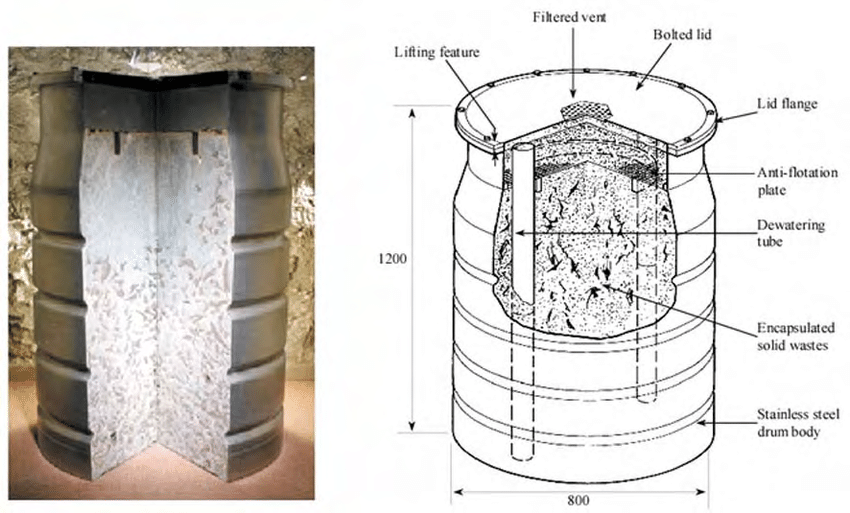
\includegraphics[scale=0.5]{Media/NuclearResearch/shows-the-500-litre-drum-waste-package-designs-The-majority-of-the-containers-are-made.png}
\caption{Cross-section of a 500L drum container labeled with materials and features \cite{500L}.}
\label{500L Drum}
\end{figure}

\begin{figure}[H]
\centering
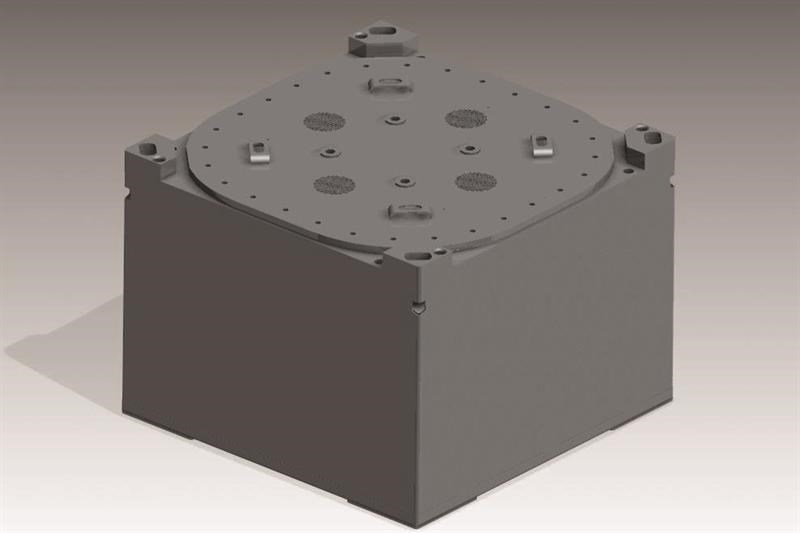
\includegraphics[scale=0.7]{Media/NuclearResearch/Pic_1_box2.jpg}
\caption{Design of a steel box container \cite{SteelBoxes}}
\label{Steel Boxes}
\end{figure}

\begin{figure}[H]
\centering
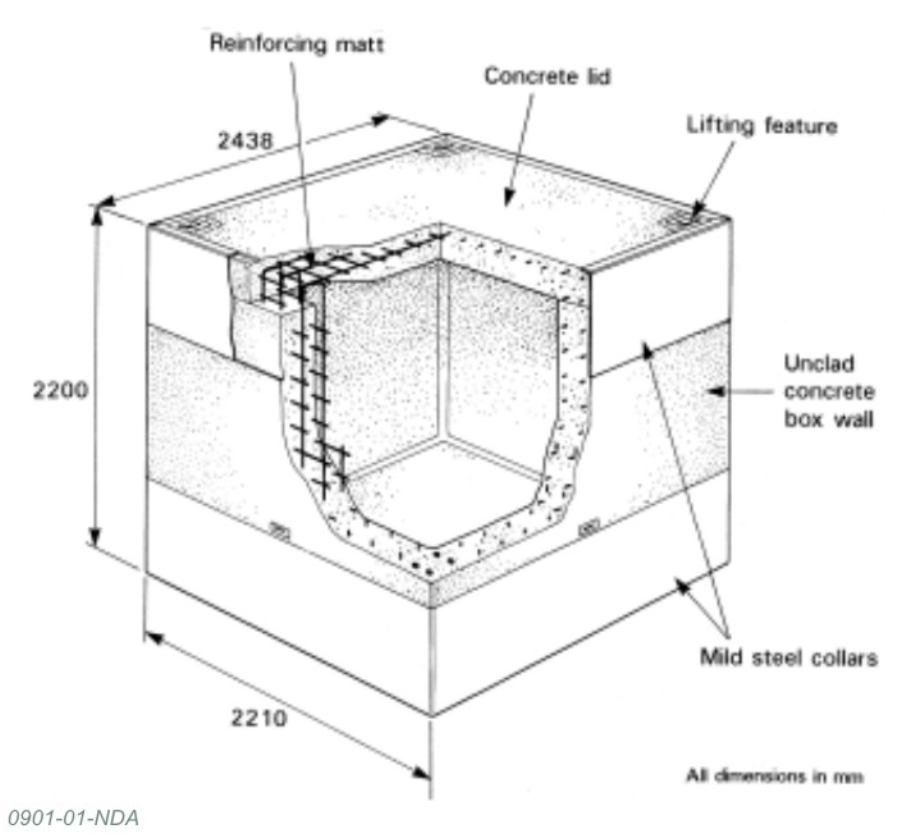
\includegraphics[scale=0.7]{Media/NuclearResearch/Screenshot 2021-03-15 at 02.54.08.png}
\caption{Cross-section of a concrete box container with its features labelled \cite{ConcreteBoxes}}
\label{Concrete Boxes}
\end{figure}

\begin{figure}[H]
\centering
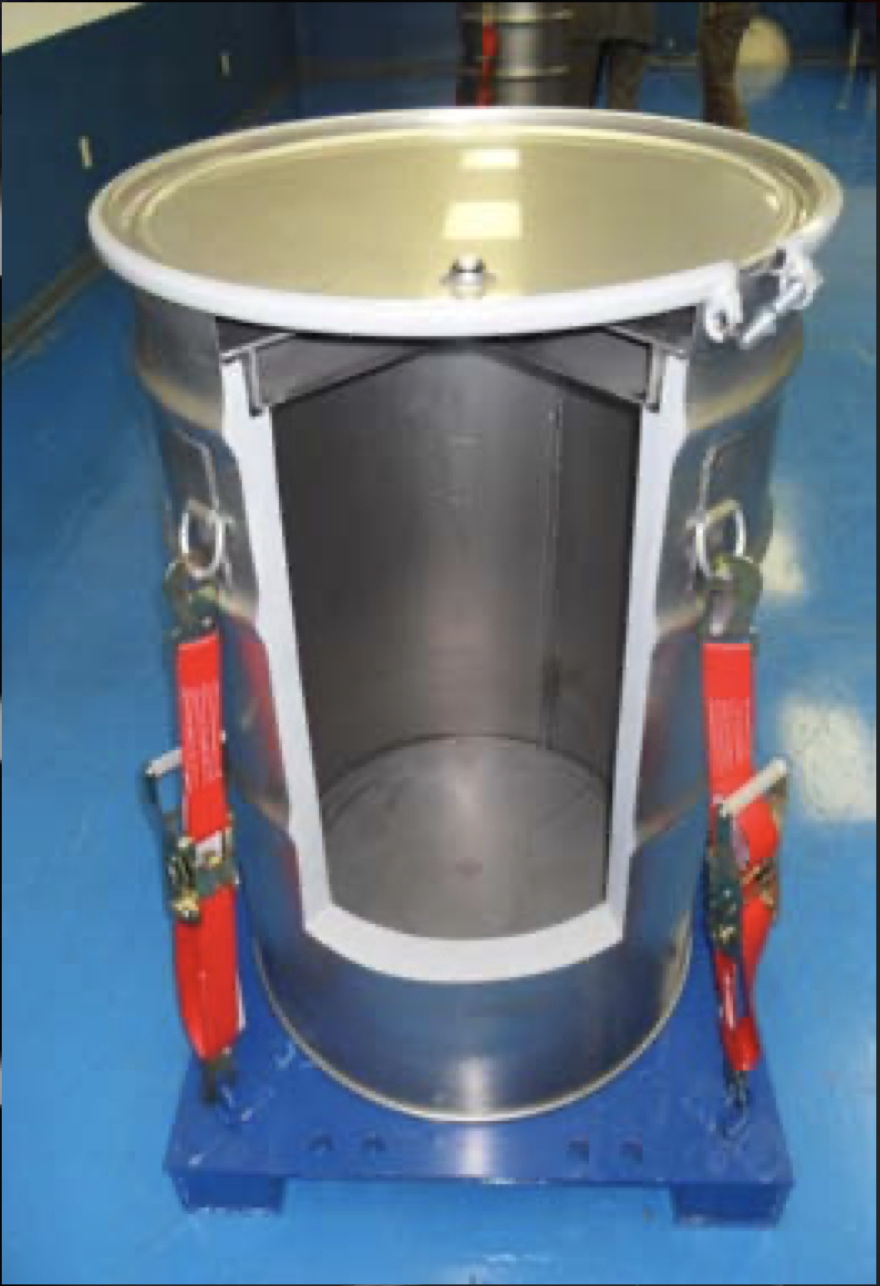
\includegraphics[scale=0.4]{Media/NuclearResearch/Screenshot 2021-03-15 at 03.18.28.png}
\caption{Cross-section of a Tru-Shield cylinder \cite{Tru-Shield}}
\label{Tru-Shield Image}
\end{figure}

\newpage
\subsubsection*{Concrete Boxes}
\label{Concrete Boxes SubSubSection}

Concrete boxes are designed for long term storage for HLW or ILW. These boxes are made from a steel frame in which concrete or high density concrete is moulded around it with steel collars to reinforce the corners, a benefit to this design is it can be lined with lead to reduce radiation penetration. The design in \cref{Concrete Boxes} implies that the concrete box houses already shielded materials, containers and due to zero ventilation, inside the concrete box must be a vacuum to provide no moisture for erosion. In reference to space saving techniques, as the boxes do not require airflow for ventilation the boxes are stack-able \cite{ConcreteBoxes}. \\

Advantages of this concrete box is that it can change physical dimension per specification and isn't time-consuming to build and serves as a permanent above ground home for ILW and HLW. Disadvantages for this container is concrete is fragile to high impacts and is soluble so water penetration can cause corrosion to the containers stored inside the concrete box so its must stay above ground in a dry and sheltered environment. Furthermore concrete can crack allowing radiation to pass more freely through if the original containers inside are compromised \cite{ConcreteBoxes}.   

\subsubsection*{Tru-Shield Cylinder}
\label{Tru-Shield Cylinder SubSubSection}

The Tru-Shield container serves as an additional shield for the 500L drums which is design to hold ILW. The design shown in \cref{Tru-Shield Image} shows a thick lead lining inside the stainless steel container and in addition further ventilation systems to further prevent radiation leaks, promoting safety in storage and transportation. These are not commonly used in the U.K, but exists to serve as a secondary container should the primary container fails i.e. a 500L drum \cite{Tru-Shield}.\\

The advantages of using the Tru-Shield is that is acts as a secondary barrier for a compromised container, it also acts as an extra safety net for if dealing with HLW. The disadvantages of this type of container is that due to the concrete box in which multiple 500L drum can be place if necessary this on contains one. This type of container serves as a temporary container for HLW due to its thick lead wall and added protection mechanics when added to the primary container.
